\section{Background}
\label{sec:background}

\subsection{Settings}
\label{subsec:settings}

\subsubsection{Stochastic Bandit Setting}

In the standard stochastic bandit setting $n = 1$. At each time step $t$, the agent takes an action $A_t \in [h]$ according to some strategies, and then it observes a random reward $r_{A_t} \in \sR$, and the mean value of $r_{A_t}$ is $r_{i, A_t}$. The agent then uses the reward to improve its action selection strategies. After such $T$ time steps, the performance of the agent's strategy is measured by the (expected) regret,
\begin{equation}
\label{eq:expected_regret}
    \r_i^{\max} \cdot T - \sE \left[ \sum\limits_{t=0}^{T-1}{  r_{i, A_t}  } \right] = \sum\limits_{t=0}^{T-1}{ \sE \left[ \tilde{r}_{i, A_t} \right] },
\end{equation}
where the expectation is taken over the randomness of action selection, if the agent is using some stochastic strategies.

Note that we choose to keep the subscript $i$ here to make the later generalization from the bandit case to the many state dependent case smoother, although there is only one state ($n = 1$) thus $i$ can be omitted without ambiguity. For simplicity, we assume $\left\| \rvs_{i} \right\|_2 = 1$, $\forall i \in [n]$.

The many state dependent stochastic bandit setting has $n > 1$, where for each state $\rvs_i$, there is a state dependent policy $\rvpi_i$. And the agent's goal is to learn totally $n$ policies using only one neural network. We assume $\left\| \rvs_{i} -  \rvs_{j} \right\|_2 \ge \delta > 0 , \ \forall i \not= j$, i.e., no duplicated data, and $\left\| \rvs_{i} \right\|_2 = 1, \ \forall i \in [n]$.

\subsubsection{Episodic Markov decision process (MDP)}

The episodic MDP setting recovers the bandit setting as a special case. The environment randomly select a starting state $\rvs_i^0 \in \sR^d$. At each time step $t$, the agent takes one action $A_t \in [h]$ according to some strategies, and then it observes a reward $r_{A_t} \in \sR$ and next state $S_{t+1} \sim \sP\left( \cdot \middle| S_t, A_t \right)$, where $\sP$ is the transition probability matrix and it is unknown to the agent. After such $H$ steps, the agent observes an ending state $S_H$, and the current trajectory terminates. At the next time step, the agent will observe a new starting state $\rvs_i^0$ randomly generated by the environment. Since we use policy gradient method (no value learning), the agent updates its NN policy weights using the cumulative reward collected after each single trajectory terminates.

\subsection{Neural Network (NN) Policy}
\label{subsec:nn_policy}

The structure of the two layer policy neural network with ReLU activation is shown in \cref{fig:nn_policy}. The policy NN takes the feature vector of each state $\rvs_i \in \sR^d$ as its input. Then it calculates the hidden node value vector by $u_{i,r} \triangleq \rvw_r^\top \rvs_i$, $\forall r \in [m]$. The logit vector is then calculated by $o_{i,k} \triangleq \rva_k^\top \sigma\left( \rvu_i \right)$, $\forall k \in [h]$, where $\sigma$ is element-wise ReLU activation function. Finally, the policy output probability is the softmax transform of the logit vector, i.e., $\rvpi_i \triangleq f\left( \rvo_i \right) = f\left( \rmA \sigma\left( \rmW \rvs_i \right) \right)$. 
\begin{figure}[t]
\vskip 0.2in
\begin{center}
\centerline{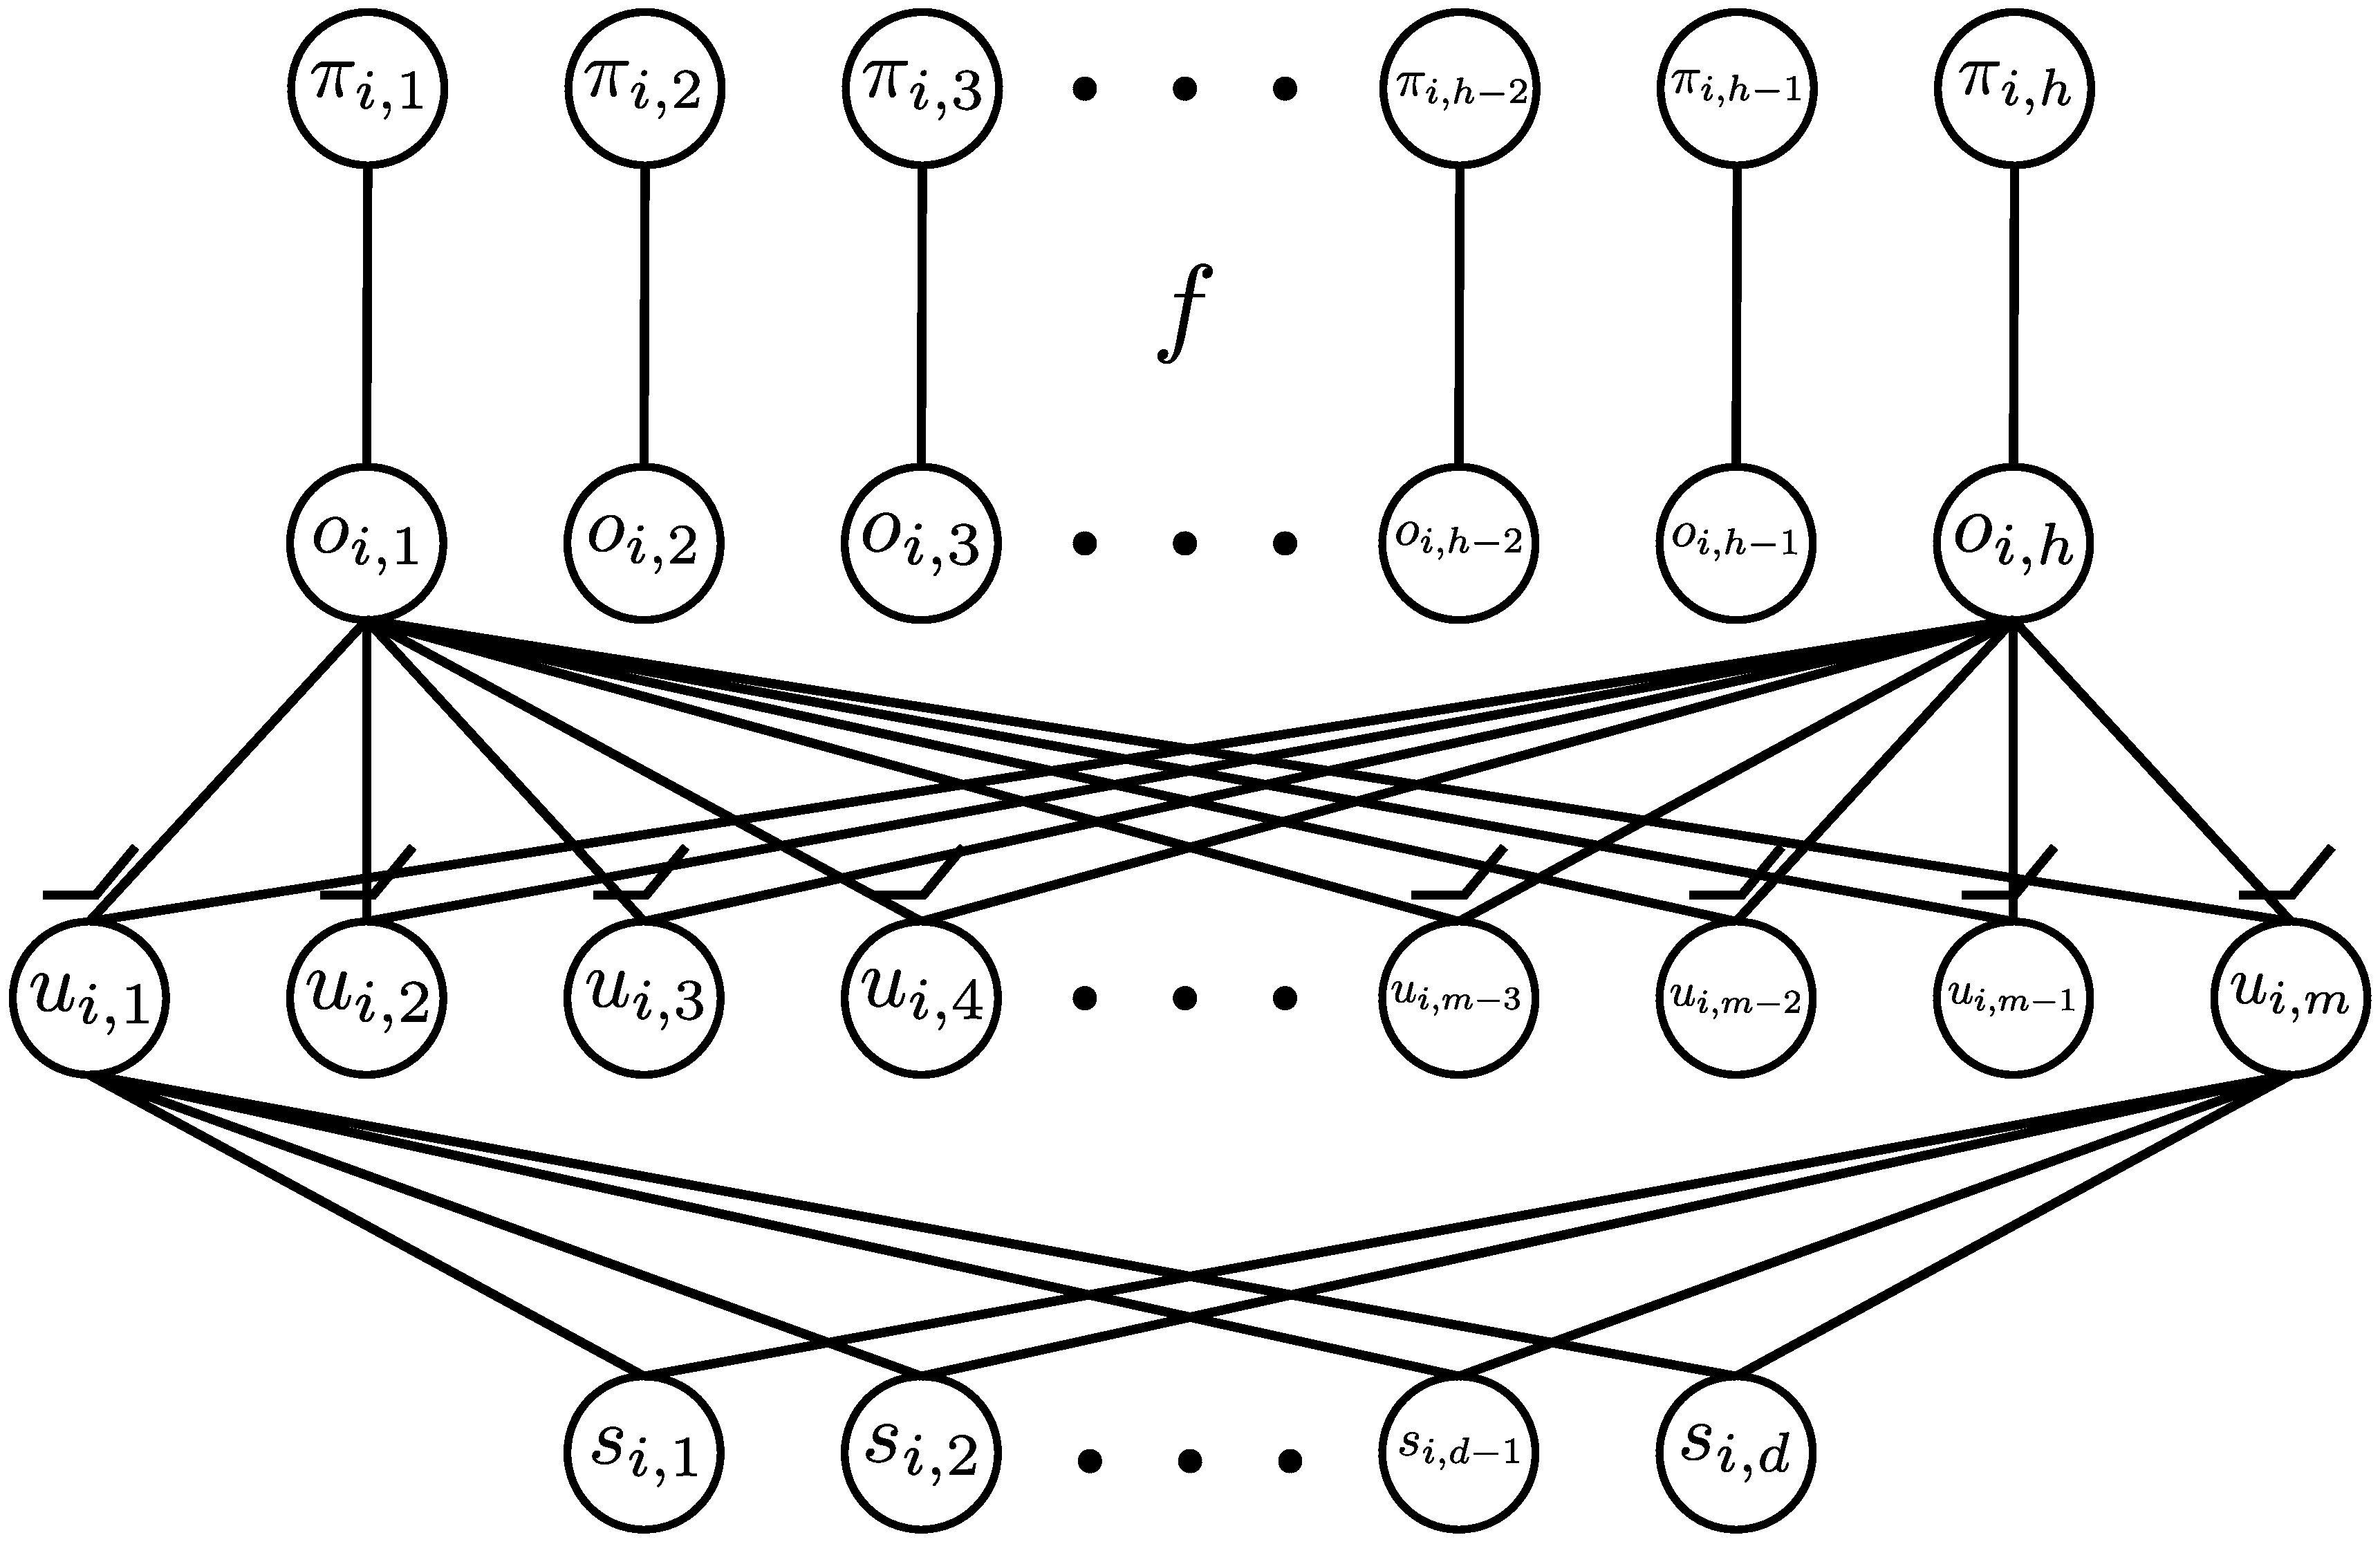
\includegraphics[width=\columnwidth]{nn_policy.pdf}}
\caption{Policy neural network.}
\label{fig:nn_policy}
\end{center}
\vskip -0.2in
\end{figure}

The above neural network defines a family of policies $\rvpi_i \left( \rmW \right)$ parameterized by $\rmW \in \sR^{m \times d}$ given any state $\rvs_i$. Let $\rvpi_i = \rvpi_i \left( \rmW \right)$, the expected loss of the NN policy can be calculated according to \cref{eq:expected_loss}.

\subsection{Vanilla Policy Gradient}
\label{subsec:vanilla_policy_gradient}

During interacting with the environment, the agent can use any strategies to select actions. In particular, if at each time step $t$, the agent's action selection strategy is the NN policy $\rvpi_i\left(\rmW(t)\right)$, then the (expected) regret is equivalent to the cumulative expected loss of $\rvpi_i\left(\rmW(t)\right)$, i.e., 
\begin{equation}
\label{eq:vanilla_policy_gradient_expected_regret}
\begin{split}
    \sum\limits_{t=0}^{T-1}{ \expectation\limits_{A_t \sim \rvpi_i\left(\rmW(t)\right)} \left[ \tilde{r}_{i, A_t} \right] } = \sum\limits_{t=0}^{T-1}{\rvpi_i\left(\rmW(t)\right)^\top \rvtilder_i},
\end{split}
\end{equation}
according to \cref{eq:expected_loss} and \cref{eq:expected_regret}. Using \cref{eq:vanilla_policy_gradient_expected_regret}, at each time step $t$, the agent can use the current NN policy $\rvpi_i\left(\rmW(t)\right)$ to sample an action, and obtain an estimation of the expected loss $\rvpi_i\left(\rmW(t)\right)^\top \rvtilder_i$. Doing policy gradient updates with respect to the NN weights $\rmW(t)$ will arguably decrease the expected loss, thus reduce the expected regret. 

However, the above mentioned method, called as vanilla policy gradient, often suffers the ``lack of exploration" problem in practice, i.e., some actions can never be explored thus cannot be learned. Unfortunately, without any other techniques, the vanilla policy gradient method cannot avoid this issue. Actually, as our analysis shown later on, the convergence rate of the policy expected loss relies on non-zero probability of exploring the optimal arms, which is consistent with intuition. For this reason, we need mix the vanilla policy gradient method with explicit exploration.

\subsection{Policy Gradient with Uniform Exploration}
\label{subsec:policy_gradient_with_uniform_exploration}

Our proposed algorithm adds explicit uniform exploration to the vanilla policy gradient method, as shown in \cref{alg:policy_gradient_uniform_exploration}. After the random initialization, at each time step $t$, one of the two cases happens. If $t < T^{\frac{2}{3} + \beta}$, then agent gets into a purely ``exploring phase", without learning the policy NN, while just collecting empirically estimated rewards. If $t \ge T^{\frac{2}{3} + \beta}$, then the agent starts ``playing and learning". The agent samples and takes actions according to the current NN policy $\rvpi_{i}\left(\rmW(t)\right)$. In the meanwhile, the agent learn the NN policy by doing policy gradient updates, with the expected empirically estimated loss calculated from the exploring phase as its objective.

\begin{algorithm}[t]
   \caption{Policy Gradient with Uniform Exploration}
\label{alg:policy_gradient_uniform_exploration}
\begin{algorithmic}
   \STATE {\bfseries Input:} State feature $\rvs_i$, learning rate $\eta > 0$, $\beta > 0$.
   \STATE Initialize $\rvw_r(0) \sim \gN\left( 0, \sigma^2 \cdot \rmI \right)$, $\forall r \in [m]$. \STATE Initialize $\rva_k \sim \gU\left\{-1, +1\right\}$, $\forall k \in [h]$.
   \STATE Initialize $\hat{r}_{i,k} = 0$, $n_{i,k} = 0$, $\forall k \in [h]$.
   \FOR{$t=0$ {\bfseries to} $T-1$}
   \IF{$t < T^{\frac{2}{3} + \beta}$}
   \STATE (Exploring Phase)
   \STATE Uniformly randomly sample action $A_{t} \in [h]$.
   \STATE Take action $A_{t}$.  Observe reward $r_{i, A_{t}}$.
   \STATE $\hat{r}_{i,A_{t}} \leftarrow \frac{\hat{r}_{i,A_{t}} \cdot 
   n_{A_{t}}}{ n_{A_{t}} + 1}$, $n_{A_{t}} \leftarrow n_{A_{t}} + 1$.
   \STATE $\rmW(t+1) \leftarrow \rmW(t)$.
   \ELSE
   \STATE (Playing-Learning Phase)
   \STATE Sample action $A_{t} \sim \rvpi_{i}\left(\rmW(t)\right)\left(\cdot \middle| \rvs_i \right)$.
   \STATE Take action $A_{t}$. Observe reward $r_{i, A_{t}}$.
   \STATE $\hat{\rvtilder}_i \triangleq \r_i^{\max} \cdot \rvone - \rvhat_i$.
   \STATE $\rmW(t+1) \leftarrow \rmW(t) - \eta \cdot \frac{d \rvpi_{i}\left(\rmW(t)\right)^\top \hat{\rvtilder}_i}{d \rmW(t)}$.
   \ENDIF
   \ENDFOR
\end{algorithmic}
\end{algorithm}

Note in \cref{alg:policy_gradient_uniform_exploration}, after the random initialization $\rva_k \sim \gU\left\{-1, +1\right\}$, $\rva_k$ is fixed, which is common in literature \citep{li2018learning,du2018gradientA,du2018gradientB,allen2018convergenceA,allen2018convergenceB}, and empirically verified that has no impact on the performance of trained NNs \citep{hoffer2018fix}. Other initialization like $\rva_k \sim \gN(0, \rmI)$ also works.

Also note that in \cref{alg:policy_gradient_uniform_exploration}, we write gradient descent over the loss objective  $\rvpi_{i}\left(\rmW(t)\right)^\top \hat{\rvtilder}_i$ for analysis. However, policy gradient update is doing gradient ascent over the reward objective $\rvpi_{i}\left(\rmW(t)\right)^\top \rvhat_i$. Actually,
\begin{equation*}
\begin{split}
    \frac{d\rvpi_{i}\left(\rmW(t)\right)^\top \hat{\rvtilder}_i}{d \rmW(t)} &= \frac{d\rvpi_{i}\left(\rmW(t)\right)^\top \left( \r_i^{\max} \cdot \rvone - \rvhat_i \right)}{d \rmW(t)} \\
    &= - \frac{d\rvpi_{i}\left(\rmW(t)\right)^\top \rvhat_i}{d \rmW(t)}.
\end{split}
\end{equation*}
Thus in practice we do not need to know $\r_i^{\max}$ and calculate $\hat{\rvtilder}_i$. It is for analysis purpose.

